\chapter{Modèle d'architecture CxSOM}
\graphicspath{{02-SOM/}}
\minitoc

En réponse à la problématique de construire des architectures décentralisées de cartes de Kohonen, nous proposons dans cette thèse une version légèrement modifiée de carte auto-organisatrices, CxSOM. L'algorithme classique d'une SOM est modifié pour permettre à une carte de prendre plusieurs entrées; la recherche du BMU est également transformée.
Nous présentons dans cette partie l'algorithme CxSOM et les paramètres utilisés.

\section{Carte de Kohonen standard}\label{sec:kohonen}
L'algorithme CxSOM est directement dérivé de l'algorithme d'une carte de Kohonen classique \cite{kohonen92}. Le principe général d'une carte de Kohonen a été décrit dans le chapitre précédent; nous définissons ici plus précisément le modèle et les équations qui serviront de base pour la définition de l'algorithme CxSOM.
\subsection{Algorithme et notations}
Une carte de Kohonen est un graphe, généralement une ligne 1D ou une grille 2D de $N$ noeuds. Nous utiliserons dans cette thèse des cartes en une et deux dimensions, c'est à dire des lignes et des grilles. Les notations et le modèle présentés ici sont toutefois applicables à des cartes de dimension et topologies quelconques.

L'algorithme et les notations sont résumés en figure~\ref{fig:one_map_not}
Les entrées sont notées $\inpx_t$, tirées dans un espace d'entrée $D$. Le poids associé à un noeud est noté $\w_e \in D$. Sa \emph{position} dans la carte est indexée par $p$. Nous choisissons d'indexer les positions entre $0$ et $1$. L'ensemble des poids est noté ${\w_e(p), p \in [0,1]}$.
Une étape $t$ de l'algorithme de mise à jour d'une carte de Kohonen est le suivant:
\begin{enumerate}
\item\label{enum:inp} Une entrée $\inpx_t$ est présentée à la carte.
\item\label{enum:act} Une \emph{activité} $a_e(\inpx_t,p)$ est calculée dans la carte. 
Cette étape est déjà une légère modification souvent utilisée de l'algorithme de Kohonen. 
Dans la version classique, les distances entre l'entrée $\inpx$ et les poids $\w(p)$ sont considérées, et le BMU est l'unité dont le poids présente la plus petite distance à l'entrée. Ici, on prendra comme BMU l'unité correspondant au maximum de l'activité.
La fonction d'activité choisie est une activation gaussienne:
\begin{equation}\label{eq:act}
a_e(\inpx_t,p) = \exp{\frac{\lVert \inpx_t-\w\ext(p) \rVert ^2}{2\sigma^2}}
\end{equation}
\item\label{enum:bmu} L'unité ayant l'activité maximale est la \emph{Best Matching Unit} de la carte. Sa position est notée $\bmu$.
\item Chaque poids $\w_e$ est déplacé vers l'entrées $\inpx$. Le déplacement est pondéré par une \emph{fonction de voisinage} $h(\bmu,p)$, dépendant de la position de chaque unité dans la carte à la best matching unit. Elle est maximale en $p = \bmu$ et décroissante autour de cette position. Dans notre étude, la fonctions de voisinage est triangulaire, donc maximales en $\bmu$, décroissante sur le \emph{rayon de voisinage} $h_e$ et nulle sinon. Cela signifie que le BMU est déplacé vers l'entrée, et les poids des unités voisines du BMU dans un rayon $h_e$ sont également déplacés, mais selon un plus faible coefficient.
\begin{equation}
\w_e(p,t+1) = \w_e(p,t) + \alpha h(\bmu,p)(\inpx_t - \w_e(p,t))
\label{eq:update}
\end{equation}
\end{enumerate}


\begin{figure}
\centering
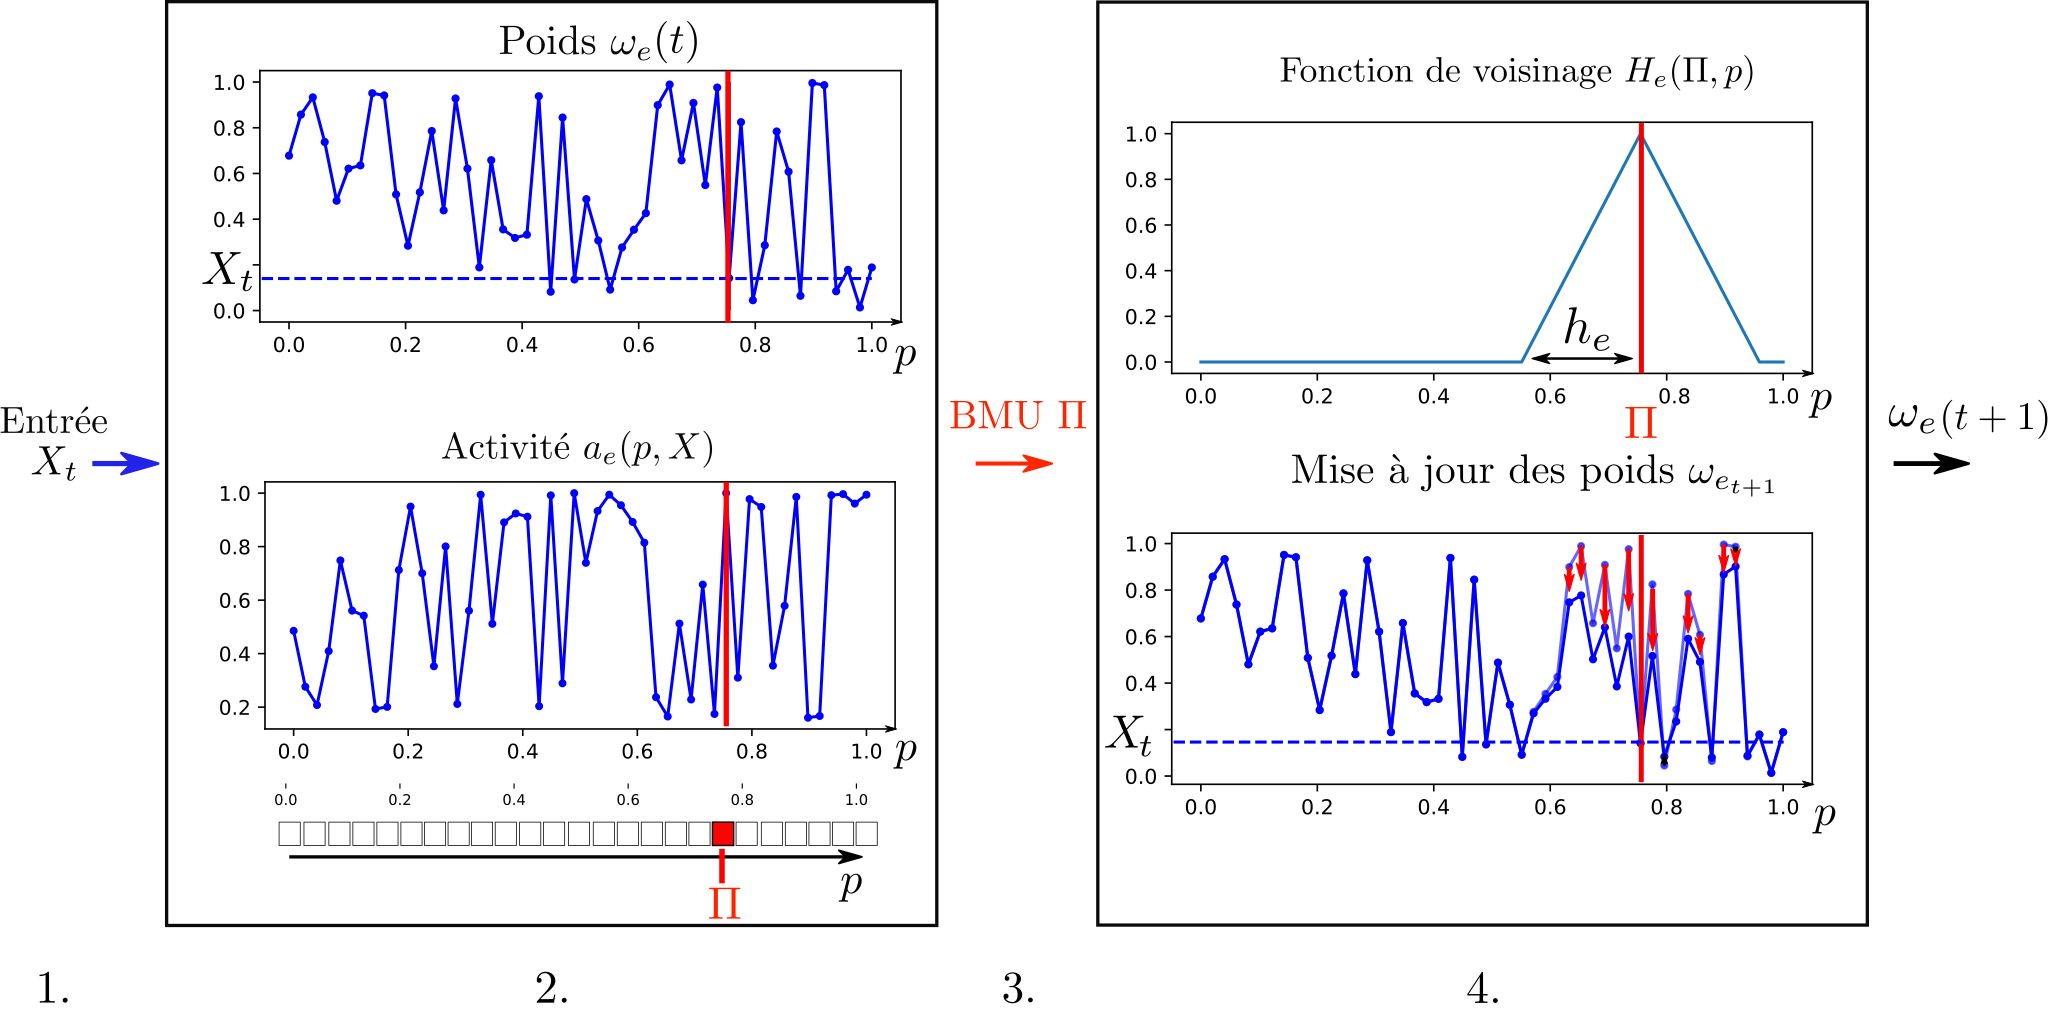
\includegraphics[width=\textwidth]{one_map_one_layer2.pdf}
\caption{Notations utilisées dans une carte de Kohonen simple}
\label{fig:one_map_not}
\end{figure}


\subsection{Paramètrage d'une carte de Kohonen}
Le dépliement d'une carte de Kohonen est géré par plusieurs paramètres. Nous détaillons ici les choix de paramètres effectués. 


\subsubsection{Taux d'apprentissage $\alpha$}

Le taux d'apprentissage $\alpha$ détermine la proportion dans laquelle chaque poids est déplacé vers l'entrée lors de sa mise à jour. Dans l'algorithme standard, le taux d'apprentissage décroit au cours de l'apprentissage. Au début de l'apprentissage, $\alpha$ est élevé, ce qui assure une organisation "grossière" rapide de la carte. $\alpha$ diminue ensuite de manière à cartographier plus localement les données. Cette décroissance assure principalement la convergence des poids de la carte au cours de l'apprentissage.
Dans l'algorithme CxSOM, nous utiliserons un taux d'apprentissage constant au cours de l'apprentissage. L'organisation des poids sera initialement un peu plus lente qu'une carte classique, mais cela permet de garder les paramètres constant au cours de l'apprentissage.
\comment{on n'aime pas les valeurs qui dépendent de $t$}
Nous observerons qu'en choisissant les bons paramètres, la convergence de la carte s'effectue correctement.
\subsubsection{Topologie de la carte}
Le graphe supportant la carte de Kohonen peut présenter diverses formes, comme détaillé en section\ref{sec:som001}. Les notations et l'algorithme CxSOM que nous présentons dans ce chapitre sont applicables à toutes les formes de cartes. Les expériences et l'évaluation du modèle se concentrent sur des lignes 1D et des grilles 2D, et omettent les formes de graphes quelconques. Ce choix est d'abord motivé par le fait que les lignes et les grilles étant les formats de cartes les plus courants rencontrés dans la littérature. On parle souvent de cartes 1D et cartes 2D lorsqu'on parle de cartes de Kohonen, en sous-entendant le format de ligne ou de grille du graphe support. Ces formes de cartes permettent de plus d'avoir une correspondance directe entre l'espace des positions $p \in [0,1]$ et un plan 1D ou 2D. Lorsqu'on parle de continuité dans une carte de Kohonen, il s'agit d'abord de proximité entre prototypes discrets. Le format de ligne et de grille permet d'étendre cette notion à une continuité des poids au sens mathématique, par interpolation. La carte est alors une fonction
\begin{equation*}
\begin{array}{ccccc}
M& : & [0,1]^2 \; \text{ou} \;[0,1] & \to & D \\
 & & p & \mapsto & \w_e(p) \\
\end{array}
\end{equation*}
Cette continuité est une des puissances d'une carte de Kohonen est est une de ses spécificité en tant qu'algorithme de quantification vectorielle. Dans le modèle CxSOM, nous traitons les positions $p$ comme un ensemble continu dans lequel faire des opérations.
Au cours de l'apprentissage, les poids d'une carte se rapprochent de la distribution des données, en gardant un ordre entre poids.
On parlera de \emph{dépliement} d'une carte pour parler de son apprentissage. Un exemple de dépliement d'une carte 1D sur des données 1D uniformément distribuées entre 0 et 1 est représenté en figure~\ref{fig:depliement}.
Dans ce cas, la carte 1D se rapproche de la fonction identité (ou moins l'identité): les poids sont ordonnés entre 0 et 1.
Ces deux configurations sont les deux seules considérées comme un bon apprentissage pour des cartes 1D sur des données 1D. Lorsque la dimension des données est plus grande que celle de la carte, par exemple des points 2D ou des images (256 dimension), la carte formera des plis de manière à remplir l'espace $D$. 

\begin{figure}
\centering
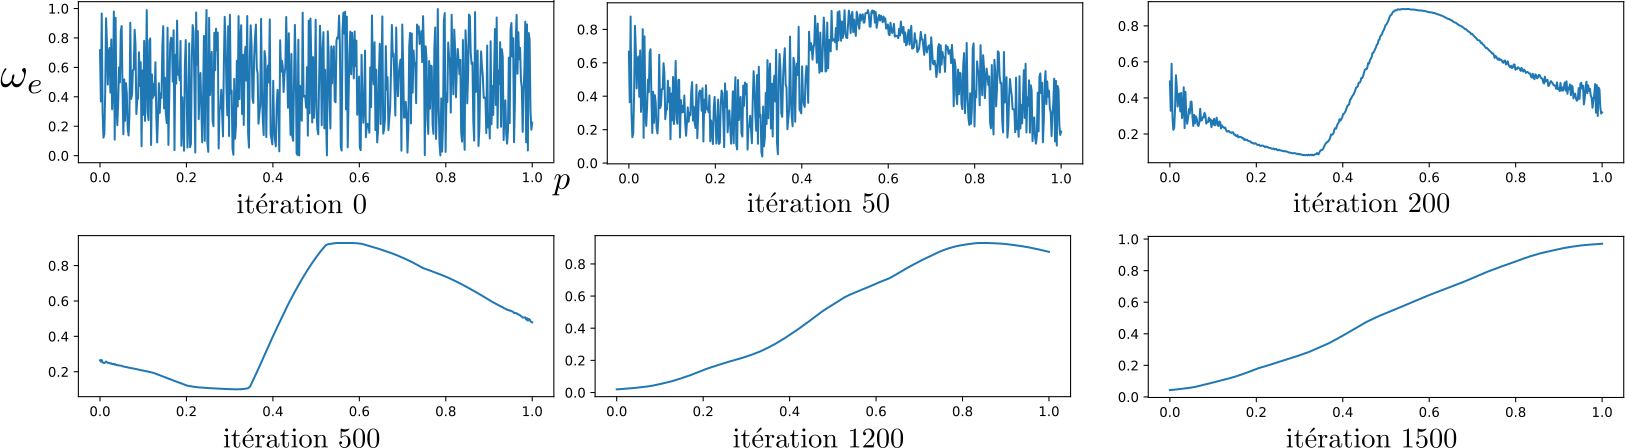
\includegraphics[width=\textwidth]{depliement_1D.pdf}
\caption{Exemple de dépliement d'une carte 1D de taille 500, sur des données 1D $\inpx \in [0,1]$. Les paramètres $h\ext = 0.2, \: \alpha = 0.2$ ont été gardé constants dans cet exemple. Une carte bien dépliée est assimilable à l'identité, comme sur cet exemple, ou moins l'identité. Ces configurations sont les deux seules pour lesquels les poids sont tous ordonnés suivant un ordre croissant ou décroissant.}
\label{fig:depliement}
\end{figure}

\subsubsection{Rayon de voisinage}
Le choix de la fonction de voisinage est déterminant dans la topologie de la carte, et en particulier le rayon de voisinage $h_e$.
Cette valeur détermine quelles unités voisines du BMU seront affectées par le déplacement du BMU.
Plus le rayon $h_e$ est grand, plus la partie de la carte déplacée vers l'entrée lors de la mise à jour est étendue. Un grand rayon d'apprentissage permet un dépliement plus rapide de la carte de Kohonen, mais l'apprentissage est peu précis car chaque poids est une moyenne d'un grand nombre de vecteurs. Les données déjà représentées sont rapidement oubliées par le déplacement des poids.
Un petit rayon d'apprentissage permet de déplacer les poids concentrés dans une petite région sans affecter toute la carte. Cela permet donc d'apprendre de nouvelles entrées sans oublier les parties déjà apprises. Par contre, utiliser un petit rayon de voisinage au début de l'apprentissage empêche une carte de bien se déplier et d'apprendre une structure globale des données. On doit donc trouver un compromis entre apprentissage de nouvelles données et mémoire des données déjà apprises.
Dans l'algorithme classique, ce compromis est trouvé en faisant décroitre le rayon de voisinage au cours de l'apprentissage. Un grand rayon de voisinage permet à la carte de se déplier rapidement en apprenant une structure globale des données. Sa décroissance permet d'affiner l'apprentissage des données à un niveau plus fin. 
Contrairement à la plupart des SOM classique, nous garderons des rayons de voisinage constants dans CxSOM. Ainsi, une étape de dépliement des cartes ne dépend pas de l'itération mais seulement de l'état précédent de la carte et de l'architecture.
%TODO citer des papiers recherchant un bon ensemble de paramètres pour l'algorithme de cartes auto-organisatrices.
\section{Modèle CxSOM}
A partir du modèle de carte de Kohonen détaillé en section \ref{sec:kohonen}, nous proposons une version de carte auto-organisatrice servant de bloc de base pour construire des architectures non-hiérarchique de cartes. Nous présentons dans cette section le modèle CxSOM. Toutes les notations et l'algorithme sont résumés en figure \ref{fig:one_map} et \ref{algo:cxsom}.

\subsubsection{Nombre de neurones d'une carte}
Le nombre de neurones d'une carte définit le niveau de quantification qu'on souhaite effectuer. Pour des opérations de classification, on choisira un nombre de neurones plus élevé que le nombre de classes, afin de pouvoir avoir plusieurs prototypes par classe.
Dans cette thèse, nous utilisons des cartes 1D comportant 500 noeuds. Le nombre de noeud est assez élevé pour pouvoir bien cartographier des ensembles de plus grande dimension. Ce nombre de noeud est proche de ce qu'on peut trouver dans la littérature.

\subsection{Choix généraux de développement}

Le modèle CxSOM étudié dans cette thèse doit permettre de construire des architectures \emph{non-hiérarchiques}. On souhaite que ce modèle soit générique, applicable à n'importe quel type d'architecture, et pouvant intégrer des connexions récurrentes. De cette manière, on ne se place pas dans une optique d'application précise mais de nouveau type de calcul. De nombreux modèles pourront être développés à partir de cette méthode. 


On définit une \emph{architecture} de carte un modèle composé de plusieurs modules qui sont chacun des cartes de Kohonen, et dans lequel des connexions sont définies entre ces éléments. Ces connexions ont un sens: on parle d'une connexions d'une carte A vers une carte B.
Dans une architecture, on peut construire un graphe $G$ orienté, dont les noeuds sont des cartes. La connexion d'une carte A vers une carte B est indiquée par la présence d'une arête de A vers B. On appelle architecture \emph{non-hiérarchique} une architecture pour laquelle $G$ n'est pas un arbre: il présente des boucles. Un exemple d'arhcitecture non-hiérarchique est représenté en figure~\ref{fig:archi_non_hierarchique}. Certaines cartes sont connectées dans les deux sens, d'autres en boucle.


Nous avons vu au chapitre précédent la notion de contexte transmise entre cartes. Dans CxSOM, on choisit de se placer dans le paradigme de transmission de la position du BMU entre cartes: on connecte une carte B à une carte A en donnant la position du BMU de B en entrée à la carte A. 
Ce paradigme de partage de positions a été utilisé dans le modèle hiérarchique HSOM~\cite{lampinen_clustering_1992}, et dans les modèles de cartes récurrentes s'appuyant sur SOMSD \cite{hammer_recursive_2004,hagenbuchner_self-organizing_2003,fix20}. Ces travaux montrent que la seule transmission d'une position de BMU permet 


L'utilisation du BMU comme contexte transmis est le paradigme choisi pour CxSOM. Contrairement aux cartes hiérarchiques HSOM dans lesquelle la position du BMU est la seule entrée d'une carte de plus haut niveau, chaque carte de l'architecture peut posséder une entrée principale propre, l'entrée \emph{externe}. L'entrée ou les entrées correspondant aux positions des BMUs d'autres cartes sont considérées comme une entrées supplémentaires d'une carte. Les cartes de Kohonen prennent donc un nombre arbitraire d'entrées, dont certaines sont les BMUs d'autres cartes. On appelle ces entrées internes à l'architecture les entrées \emph{contextuelles} d'une carte.
L'algorithme d'apprentissage d'une carte auto-organisatrice e l'architecture est le même qu'une carte classique, comprenant:
\begin{enumerate}
\item\label{etape:entree} Présentation de son entrée à la carte 
\item\label{etape:bmu} Recherche du BMU par calcul d'activité
\item\label{etape:maj} Mise à jour des poids selon une fonction de voisinage
\end{enumerate}

Chaque carte aura maintenant plusieurs entrées: une entrée \emph{externes} dans un espace d'entrée, facultative, et $k$ entrées \emph{contextuelles} qui sont les positions des BMUs des cartes qui lui sont connectées. 
La recherche du BMU doit être modifiée par rapport à la méthode originale : les rétroactions entre les cartes sont autorisées, la position du BMU de la carte A va donc influencer la position du BMU de la carte B, lequel modifie à nouveau le BMU de la carte A, etc. 


Notre algorithme implémente donc deux modifications principales par rapport à l'algorithme d'apprentissage d'une carte de Kohonen classique: 
\begin{itemize}
\item Les cartes possèdent plusieurs entrées, externes et contextuelles; les entrées contextuelles sont les positions des BMUs d'autres cartes. Le calcul de l'activité est modifié afin de prendre en compte ces différentes couches d'entrées.
\item La recherche du BMU est modifiée afin de gérer les rétroactions entre cartes.
\end{itemize}

La description du modèle CxSOM est détaillée en figure~\ref{fig:one_map}, dans un cas ou une carte reçoit deux connexions, et l'algorithme explicité en~\ref{algo:cxsom}.

\begin{figure}
\centering
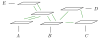
\includegraphics[width=0.6\textwidth]{architecture.pdf}
\caption{Exemple d'architecture modulaire \emph{non-hiérarchique} de cartes de Kohonen. Les entrées sont $A,B,C,D,E$ quelconques. Chaque carte peut ou non prendre une entrée ; les connexions sont réciproques ou non.}
\label{fig:archi_non_hierarchique}
\end{figure}

\subsection{Connexion entre cartes}
A un pas d'apprentissage $t$, une carte $M$ reçoit en entrée une entrée \emph{externe} notée $\inpx_t$ et $K$ entrées \emph{contextuelles} notées $\inpc_{0t},\cdots,\inpc_{Kt}$, qui sont les positions des BMU $\bmu$ des cartes qui lui sont connectées. La carte possède donc $k+1$ couches de poids. $\w_e$ correspond à l'entrée externe et $\w_{c0}, \cdots, \w_{cK}$ aux entrées contextuelles. On calcule une activité séparément sur chaque couche de poids selon la formule suivante : 
\begin{equation}
\label{eq:activite}
a(p,x) = \exp(\frac{(\w(p)-x)^2}{2\sigma^2} \; x = \inpx_t\; \text{ou}\; \inpc_{kt}, \; \w = \w_e \;\text{ou}\; \w_{ck}
\end{equation}
Les activités contextuelles sont moyennées en une activité $a_c(p,\mathbf{\inpc}_t)$, avec $\mathbf{\inpc_t} = (\inpc_{0t}, \cdots, \inpc{Kt})$. 
Les activités externes et contextuelles sont enfin fusionnées en une activité globale:
\begin{equation}
\label{eq:global_act}
a_g(p,\inpx_t,\mathbf{\inpc_t}) = \sqrt{a_e(p,\inpx_t)(\beta a_e(p,\inpx_t) + (1-\beta) a_c(p, \mathbf{\inpc_t})}
\end{equation} 

\begin{figure}
\centering
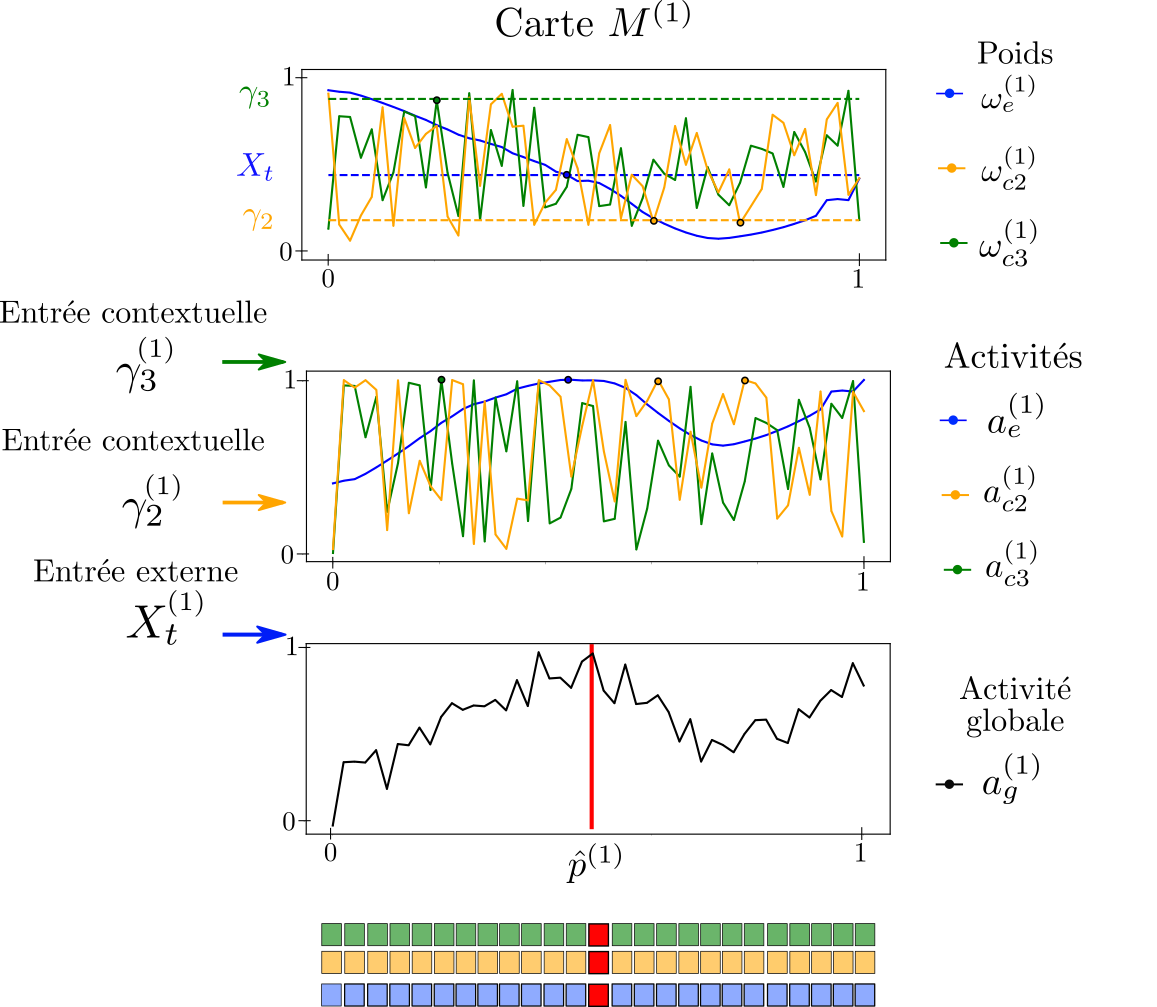
\includegraphics[width=0.8\textwidth]{activite_layers.pdf}
\caption{Calcul d'activité dans une SOM prenant plusieurs entrées au sein d'une architecture : une entrée externe et deux entrées contextuelles. L'indice $(1)$ permet de distinguer les objets relatif à cette carte. Les entrées externes sont $X\m{1}_t$. les deux entrées contextuelles sont $\inpc\m{1}_2$ et $\inpc\m{1}_3$. La carte possède trois couches de poids, permettant de calculer trois activités. L'activité globale prend en compte tout les couches d'activités afin de trouver un BMU commun pour toutes les couches de poids. Ce calcul favorise l'activité externe et est modulé par les activités contextuelles, ce qu'on observe sur la courbe du bas. Le maximum de l'activité globale est noté $\hat{p}$. A partir de l'activité globale, le BMU $\bmu\m{1}$ sera trouvé par le processus de relaxation décrit en partie suivante.}
\label{fig:activite}
\end{figure}

\subsection{Calcul du BMU par relaxation}

Contrairement à une carte simple, on ne peut pas calculer tous les BMUs de l'architecture d'un coup en prenant l'argmax de $a_g$ dans chaque carte.
A cause des influences mutuelles entre cartes, calculer le BMU d'une des cartes modifie les entrées des autres cartes de l'architecture, et donc leur BMU. 
On remplace donc l'étape de calcul d'argmax par un processus global à l'architecture de recherche de BMU. On cherche, dans chaque carte $i$, la position $\bmu\m{i}$ telle que $\forall i, a_g\m{i}(\bmu\m{i},\inpx\m{i},\bmu\m{i_0},\cdots,\bmu\m{i_k})$ soit maximale.
Cette recherche est réalisée par un processus dynamique que l'on appelera \emph{relaxation}, menant à un consensus entre cartes : on cherche un point, s'il en existe, où le BMU de chaque carte est au plus proche de son activité globale. On remplace l'étape de calcul d'argmax par le processus de relaxation.

Le processus de relaxation est une boucle imbriquée dans un pas d'apprentissage de l'architecture, indexée par $\tau$. Notons $\bmu\m{i}$ la position du BMU de la carte $i$, et $\mathbf{\bmu} = (\bmu\m{0}, \cdots , \bmu\m{n})$, avec $n$ le nombre de cartes de l'architecture.
Au début d'un pas d'apprentissage, chaque carte est nourrie avec une entrée externe, donc $\inpx\m{i}_t$ les activités externes $a_e\m{i}(\inpx\m{i}_t,p)$ de chaque carte peuvent être calculées.
La recherche du BMU suit le processus de relaxation suivant :
\begin{enumerate}
\item Dans chaque carte $i$, la position $\bmu\m{i}$ est initialisée à $\hat{p}\m{i}_0 = \argmax_{p\m{i}}(a_e\m{i}(\inpx\m{i}_t,p)$. Les entrées contextuelles de chaque carte peuvent ainsi être attribuées.
\item Tant que toutes les positions $\bmu\m{i}$ ne sont pas stables, 
	\begin{enumerate}
	\item Dans chaque carte $i$, calculer les activités contextuelles et globales, définissant ainsi $\hat{p}\m{i}_\tau = \argmax_{p\m{i}}(a_g\m{i}(p\m{i},\inpx\m{i}, \bmu\m{i_0}_\tau,\cdots,\bmu\m{i_k},_\tau)$, avec $i_0, \cdots, i_k$ les indices des cartes connectées à $i$ dans l'architecture.
	\item Déplacer $\bmu\m{i}$ vers $\hat{p}\m{i}$ : $\bmu\m{i}_{\tau +1} \leftarrow \bmu\m{i}_\tau \pm \Delta$ si $\lvert \bmu\m{i}- \hat{p}\m{i}\rvert \geq \Delta$, $\bmu^i \leftarrow p^{\star i}$ sinon
	\end{enumerate}
\item Le BMU de chaque carte est pris comme la valeur finale stable de ce processus dynamique. Cette valeur est utilisée pour les mise a jour des poids.
\end{enumerate}

Il peut arriver que les positions se stabilisent sur un cycle limite. Dans ce cas, on arrêtera la relaxation arbitrairement; ce phénomène étant ponctuel, il n'influence pas l'apprentissage. Les paramètres des cartes de l'architecture sont choisis pour éviter de telles situations.

\begin{figure}
\centering
\includegraphics[width=0.6\textwidth]{relaxation.pdf}
\label{fig:relax}
\caption{description d'une étape de la relaxation dans l'architecture, aboutissant à un consensus entre cartes. Au sein d'une même itération $t$, les position des BMU $\bmu$ sont légèrement déplacées jusqu'à ce que toutes les positions $\bmu$ des cartes de l'architecture soient stable. Ces positions maximisent collectivement les activités globales de chaque carte. }
\end{figure}

\begin{figure}
\centering
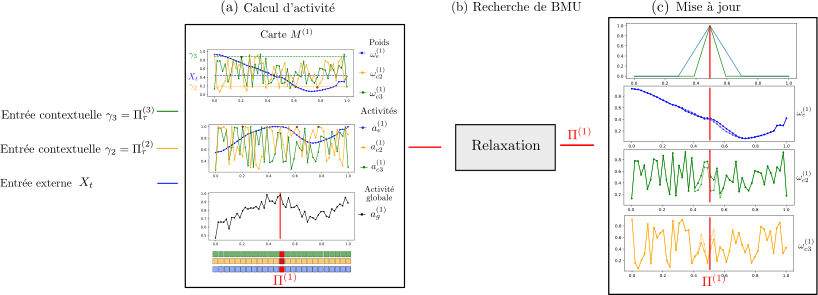
\includegraphics[width=\textwidth]{map_2layers.pdf}
\caption{Description d'une carte au sein d'une architecture CxSOM. La carte recoit deux connexions de cartes voisines, et possède donc deux couches contextuelles}
\label{fig:one_map}
\end{figure}

\subsection{Mise à jour des poids}

Les poids sont mis à jour par rapport à leurs entrées respectives suivant l'équation \ref{eq:update}. Le BMU d'une carte est ainsi commun à toutes les couches. Les rayons de voisinage $h_e$ et $h_c$ ont des valeurs différentes ; celles-ci seront détaillée en partie suivante. 
Il faut noter que les poids contextuels cartographient l'espace des positions d'une autre carte. Les positions des cartes sont donc associées par les poids contextuels.

\begin{figure}
\begin{minipage}[c]{0.5\textwidth}
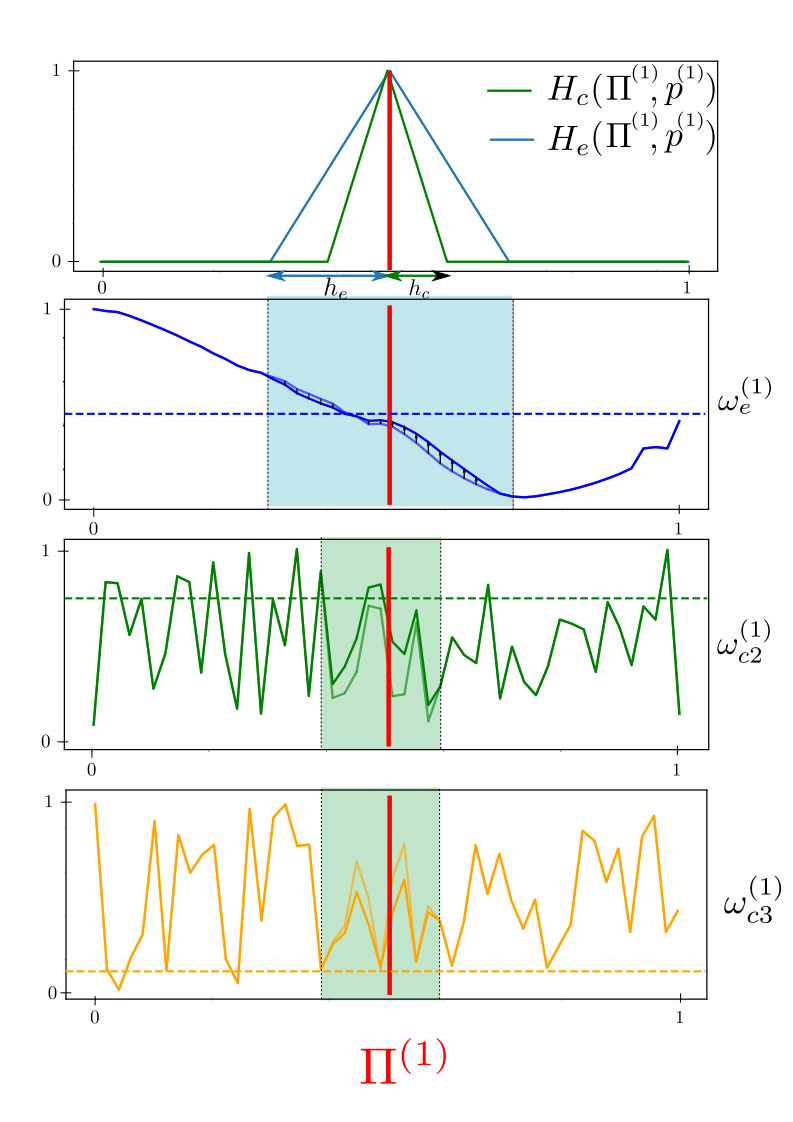
\includegraphics[width=\textwidth]{maj_layers.pdf}
\end{minipage}
\hfill
\begin{minipage}[c]{0.4\textwidth}
\caption{Mise à jour de chaque couche de poids indépendamment, relativement au BMU commun $\bmu\m{1}$. Le rayon de voisinage $h_e$ est utilisé pour mettre à jour les poids externes, le rayon $h_c$ pour mettre à jour les poids contextuels. On choisit $h_e > h_c$. Cette différence permet une différence d'échelle d'apprentissage entre couches de poids. Elle est détaillée en section suivante.}
\end{minipage}
\label{lig:maj}
\end{figure}
\subsection{Etape de test et prédiction d'entrée}

\subsection{Résumé : Algorithme général}

\begin{algorithm}\label{algo:relax}
\caption{Pas d'apprentissage $t$}
\SetAlgoLined
  \KwData{$\inpx\m{1}_t, ... , \inpx\m{K}_t$ tirés dans $\mathcal{D}\m{1} \times \cdots \times \mathcal{D}\m{n}$}
  $\tau \leftarrow 0$ \;
  \lForEach{Carte $i$}{$\bmu\m{i}_0 \leftarrow \argmax_{p\m{i}} a\ext(\inpx\m{i}_t,p\m{i})$}
  \While {$\mathbf{\bmu}_\tau \neq \mathbf{ \bmu}_{\tau-1}$ et $\tau < N_{max}$}{
  \ForEach{Carte $i$}{
  $\inpc\m{i}_1,...\inpc\m{i}_k \leftarrow \bmu\m{i_0}_\tau, \cdots, \bmu\m{i_k}_\tau$, $i_0, \cdots i_k$ indices des cartes connectées à $i$ dans l'architecture \;
	Calcul de $a_{c1}\m{i}(\inpc_1,p\m{i}), \cdots, a_{ck}\m{i}(\inpc_k,p\m{i})$ \;
  	Calcul de $a_g\m{i}(\inpx\m{i}, \bmu\m{i_0}_\tau, \cdots, \bmu\m{i_k}_\tau)$ (equation~\ref{eq:global_act}) \;
  $\hat{p}\m{i}_\tau = \argmax_{p\m{i}} a_g\m{i}(\inpx\m{i}, \bmu\m{i_0}_\tau, \cdots, \bmu\m{i_k}_\tau)$ \;
  Déplacement de $\bmu\m{i}_\tau$ vers $\hat{p}\m{i}$ d'un pas $\Delta$:
  $\bmu\m{i}_{\tau+1} \leftarrow \bmu\m{i}_\tau + min(\Delta, \lvert \hat{p}\m{i} - \bmu\m{i} \rvert) \times \sign(\hat{p}\m{i} - \bmu\m{i})$ \;
  }
  $\tau \leftarrow \tau + 1$ \;
  }
  $\bmu\m{1}, \cdots, \bmu\m{n} \leftarrow \hat{p}\m{1}_\tau, \cdots , \hat{p}\m{n}_\tau$ \;
  \ForEach{Carte $i$}{
  $\w\ext\m{i}(p) \leftarrow \w\ext\m{i}(p) + H\ext(\bmu\m{i}, p)(\w\ext\m{i}(p) - \inpx\m{i})$ \;
  \lForEach{$k$}{$\w_{ck}\m{i}(p) \leftarrow \w_{ck}\m{i}(p) + H\cont(\bmu\m{i},p)(\w_{ck}\m{i}(p) - \inpc\m{i})$}
  }
 \end{algorithm}
 
 \begin{algorithm}
\caption{Etape de test}
\SetAlgoLined

 \end{algorithm}
 
  \begin{algorithm}
\caption{Etape de Prédiction}
\SetAlgoLined
\KwData{$m$, indice de la carte servant à faire de la prédiction}

 \end{algorithm}

 

\section{Choix des paramètres}

\subsection{Paramètrage d'une carte}
On retrouve les mêmes paramètres dans CxSOM que sur une carte classique: taille de la carte, topologie et dimensions. 
Contrairement à une carte simple, on a maintenant un jeu de paramètre d'apprentissage par couche de poids d'une carte : pour chaque couche de poids $\w_e$ et $\w_{ck}$, on peut faire varier le taux d'apprentissage $\alpha$ et le rayon de voisinage $h_e$ ou $h_c$.
On choisit de prendre un taux d'apprentissage $\alpha$ commun à toutes les couches dans un souci de simplicité. $\alpha$ restera constant au cours de l'apprentissage, contrairement à une carte classique dans laquelle $\alpha$ décroît.
On choisit également de prendre des valeurs $h_{ck}$ communes à toutes les couches de poids contextuelles. Ainsi, on apporte une symétrie dans les connexions: les carte réagissent de la même façon aux autres cartes.
Par contre, on choisit de prendre le rayon externe $h_e$ très supérieur au rayon contextuel. Ce choix de paramètres apporte deux échelles de vitesse dans l'apprentissage, sans avoir à modifier les paramètres au cours du dépliement. Les poids externes se déplient alors très rapidement sur les données, quand les poids contextuels se déplacent très peu au début. Lorsque les poids externes sont organisés, l'apprentissage n'influence plus que les poids contextuels et ces derniers se déplient. 


\subsection{Paramètres de l'architecture}

